\begin{mainquestion}{sourcetransform}{Source Transformations}
Use source transformations to find the voltage $V_{O}$ in the circuit below.

\begin{center}
    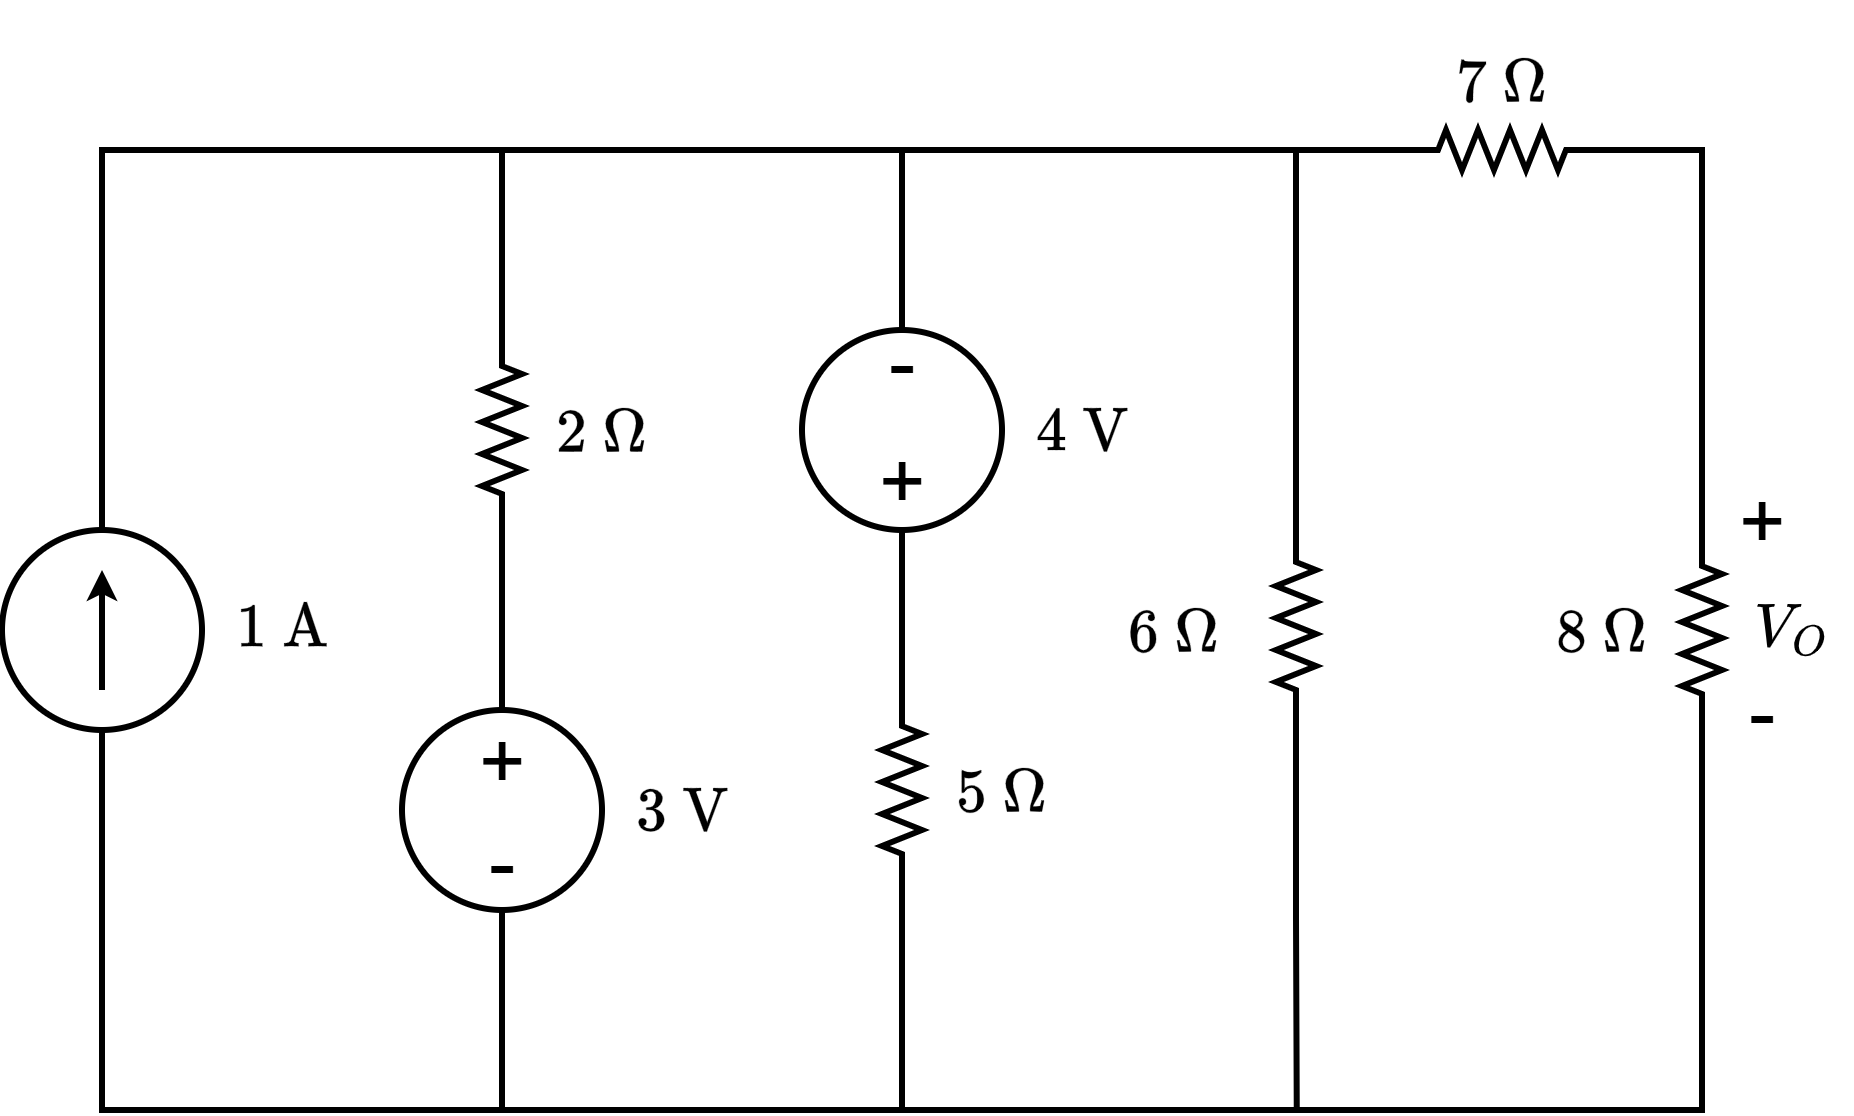
\includegraphics[width=5.2in]{circuit.png}
\end{center}

\begin{partquestion}{findvo}{Find $V_{O}$ using source transformations.}
\begin{answer}
We first transform the 3 V source with the $2~\Omega$ series resistance into its Norton equivalent with a Norton source current of $\frac{\qty{3}{\volt}}{\qty{2}{\ohm}} = \qty{1.5}{\ampere}$ and a Norton resistance of $2~\Omega$. Simultaneously, we can transform the 4 V source with the $5~\Omega$ series resistance into its Norton equivalent with a Norton source current of $\frac{\qty{4}{\volt}}{\qty{5}{\ohm}} = \qty{0.8}{\ampere}$
and a Norton resistance of $5~\Omega$. Note the polarity of the two sources are different, so the Norton current sources will be pointing in different directions! The resulting circuit looks like:

\begin{center}
    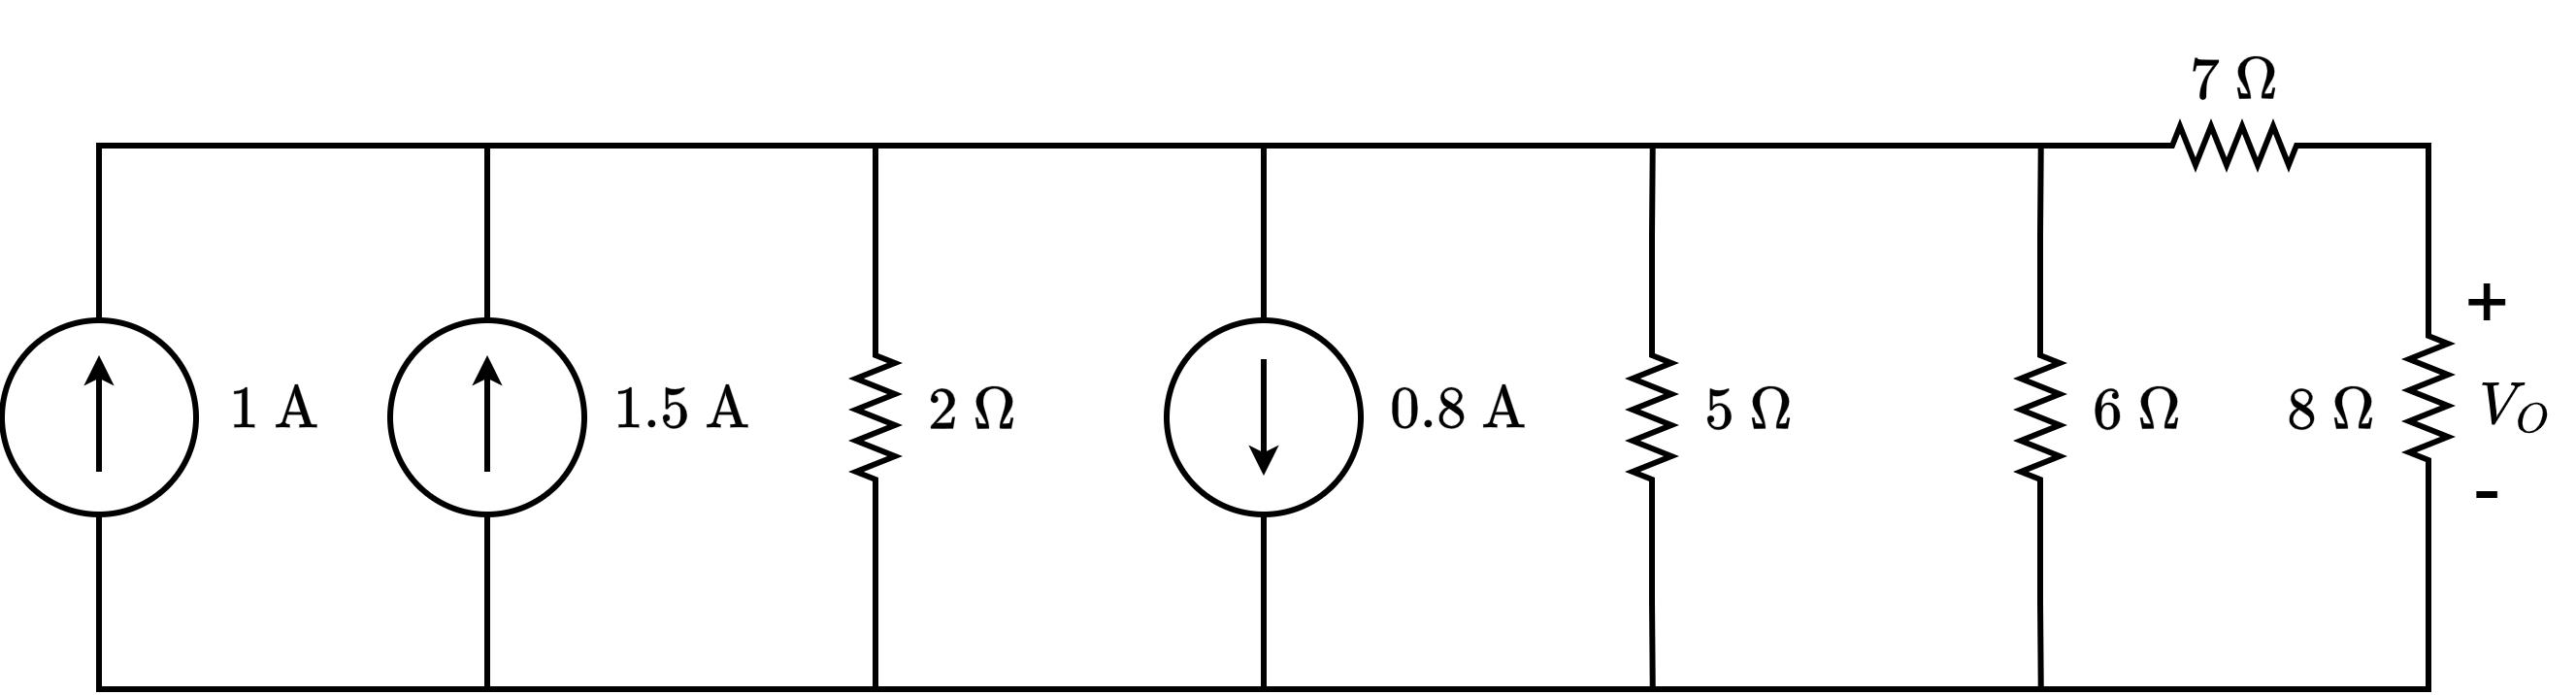
\includegraphics[width=0.8\textwidth]{transform_1.png}
\end{center}

We can simplify the circuit considerably by combining the current sources since they are in parallel to form a $\frac{17}{10}\unit{\ampere}$
source. We can also combine the three parallel resistors with a single resistor of value $\frac{15}{13}\unit{\ohm}$
The simplified circuit looks like:

\begin{center}
    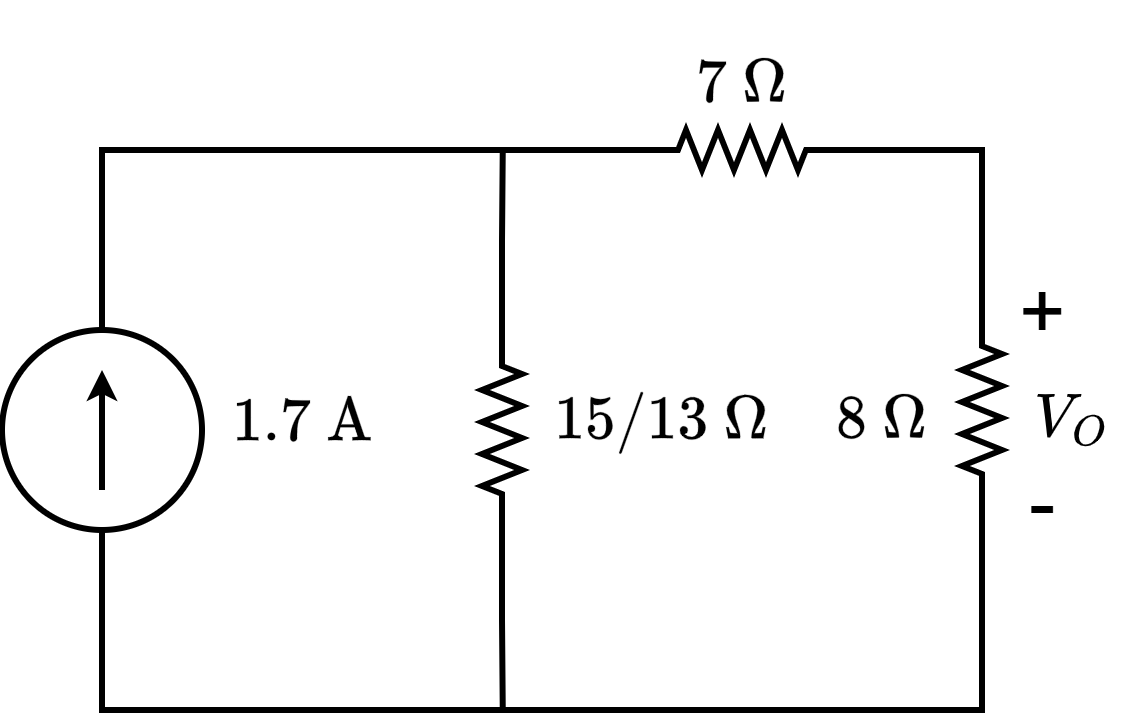
\includegraphics[width=0.5\textwidth]{transform_2.png}
\end{center}

The next step is to apply another source transformation to a Thévenin equivalent with a Thévenin voltage source of $\frac{51}{26}\unit{\volt}$
with a Thévenin resistance of $\frac{15}{13}\unit{\ohm}$.
The result looks like:

\begin{center}
    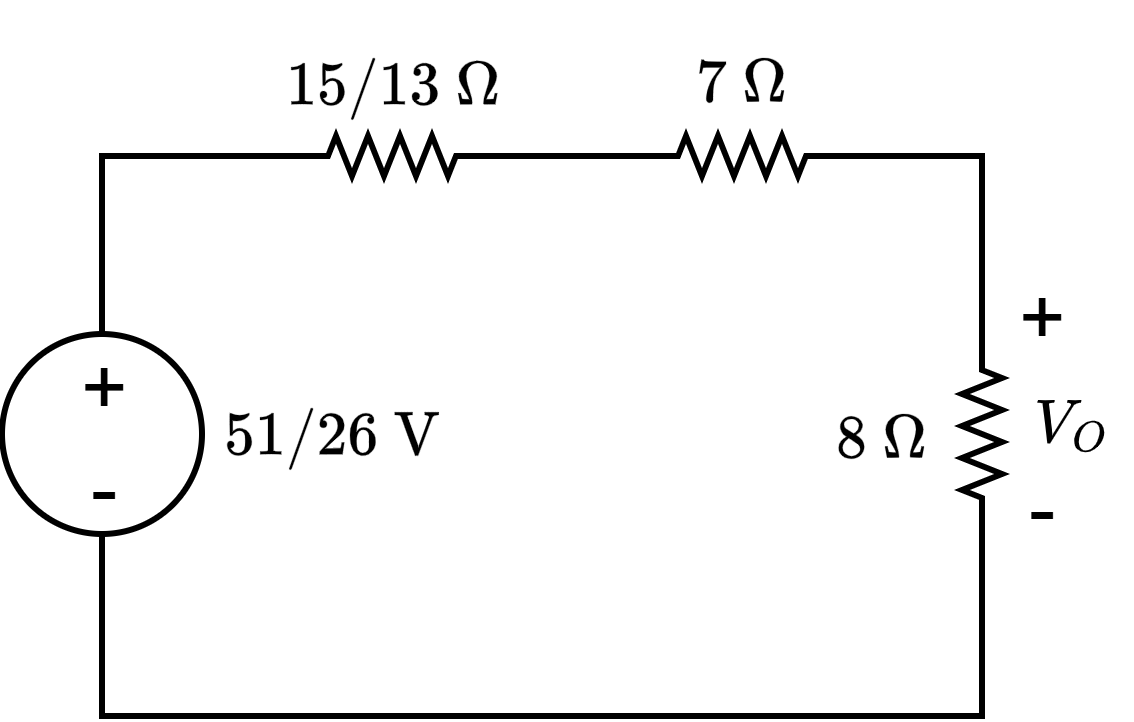
\includegraphics[width=0.5\textwidth]{transform_3.png}
\end{center}

The result is a simple voltage divider. We can easily find the voltage across the $8~\Omega$ resistor as:
\[
V_{O}
=
\frac{51}{26}
\left(
\frac{8}{8+\frac{15}{13}+7}
\right)
=
\frac{34}{35}\,\si{\volt}.
\]
\end{answer}
\end{partquestion}

\end{mainquestion}